%-----------------------------------------------------------------------------
% Schriftgr��e, Layout, Papierformat, Art des Dokumentes
%-----------------------------------------------------------------------------
\documentclass[12pt,					% Grundschriftge
							 oneside,			% einseitiges Dokument
							 a4paper,			% Papiergr��e
							 halfparskip,		% Einzug bei einem Absatz
							 liststotoc,			% Verzeichniss (Abbildungen erc.) in das Inhaltverzeichnis
							 bibtotoc,			% Literaturverzeichnis ins Inhaltverzeichnis
							 fleqn,				% Mathematische Formeln linksb�ndig darstellen
							 pointlessnumbers]	% Punkt am Ende der Nummerierung des Inhaltsverzeichnisses 													entfernen
							 {scrreprt}

%-----------------------------------------------------------------------------
% Konstanten festlegen
%-----------------------------------------------------------------------------
\newcommand{\VerfasserJ}{Josef Prothmann}
\newcommand{\EmailJ}{j.prothmann@stud.hs-wismar.de}
\newcommand{\GeburtstagJ}{16. Dezember 1998}
\newcommand{\GeburtsortJ}{Dannenberg/ Elbe}

\newcommand{\VerfasserD}{David Oliver Taube}
\newcommand{\EmailD}{d.taube@stud.hs-wismar.de}
\newcommand{\GeburtstagD}{9. Februar 1994}
\newcommand{\GeburtsortD}{Rostock}


\newcommand{\Titel}{Entwicklung eines User Interfaces f\"ur einen serverbasierten, 3D gedruckten Roboterarm}
\newcommand{\Betreuer}{Prof. Dr. H. Litschke}



\newcommand{\blankpage}{
%	\newpage
%	\thispagestyle{empty}
%	\mbox{}
	\newpage
}

%-----------------------------------------------------------------------------
% verwendete Pakete
%-----------------------------------------------------------------------------
\usepackage[utf8]{inputenc}		% Zeichkodierung , Umlaute erlauben
\usepackage[T1]{fontenc}				% Wahl des Fonts, bzw. der Kodierung
\usepackage[english,ngerman]{babel}		% neue deutsche Rechtschreibung verwenden
\usepackage{graphicx}					% erm�glicht das Einbinden von Grafiken, sehr wichtig!
\usepackage{fancyhdr}					% f�r formatierte Kopf- und Fu�zeilen
\usepackage{setspace}					% Package zum Kontrollieren von Leerr�umen
\usepackage{subfigure}					% erweiterte Darstellung von Bildern
\usepackage{listings}					% M�glickeit zum Anzeigen von Quelltexten
\usepackage{color,moreverb}				% Farben
\usepackage{lmodern}					% bietet neuere Schriften, sieht besser aus im Acrobat Reader
\usepackage{amsmath,amssymb}			% erweiteter Formelsatz und zus�tzliche Mathe-Symbole
\usepackage{booktabs}					% professionelle, typographisch richtige Tabellen
\usepackage{cite}						% f�r LibTex
%\usepackage{shortvrb}					% f�r Quellcode mit \begin{verbatim}
\usepackage[binary-units=true]{siunitx}	% Darstellung von Si-Einheiten
%\usepackage{pdfpages}					% pdf-Seiten einbinden
\usepackage{enumitem}					% custom itemiziation




%-----------------------------------------------------------------------------
% Fu�notennummerierung nicht f�r jedes kapitel zur�cksetzen
%-----------------------------------------------------------------------------
\usepackage{chngcntr}
\counterwithout{footnote}{chapter}

%-----------------------------------------------------------------------------
% Einstellungen der Seitenr�nder
%-----------------------------------------------------------------------------
\usepackage[left=3cm,						% linker Rand
						right=3cm,			% rechter Rand
						top=1.5cm,			% oberer Rand
						bottom=1.5cm,		% unterer Rand
						includeheadfoot,	% bezieht die Kopf- und Fu�zeile mit ein
						bindingoffset=0cm]	% Bundsteg
						{geometry}



%-----------------------------------------------------------------------------
% Daten f�r die Titel des Artikels
%-----------------------------------------------------------------------------
\title{Praktikumsbericht}
\author{\Verfasserj \VerfasserD}
\date{\today{}}

%-----------------------------------------------------------------------------
% Metadaten in pdf einf�gen
%-----------------------------------------------------------------------------
\usepackage[pdftex,
						pdfauthor={\VerfasserJ},									% Name des Autors
						pdftitle={\Titel},										% Name der Arbeit
						pdfcreator={MiKTeX, LaTeX with hyperref and KOMA-Script},	% Von was erzeugt
						pdfsubject={Praktikumsbericht},							% Was f�r eine Arbeit ist es
						pdfkeywords={\Titel},
						plainpages=false,
						hypertexnames=false,
						pdfpagelabels]{hyperref}

%-----------------------------------------------------------------------------
% Schriftarten anpassen
%-----------------------------------------------------------------------------
\setkomafont{sectioning}{\rmfamily\bfseries}			% Titelzeilen
\setkomafont{caption}{\small}							% Schrift f�r Caption
\setkomafont{captionlabel}{\sffamily\bfseries\small}	% Schrift f�r 'Abbildung'
\setkomafont{chapterentry}{\small\bfseries}				% Schrift f�r Inhaltsverzeichnis
\setkomafont{chapter}{\large\bfseries}					% Schrift f�r Kapitel
\setkomafont{section}{\normalsize}						% Schrift f�r Section
\setkomafont{subsection}{\normalsize}					% Schrift f�r Subsection
						



				
%-----------------------------------------------------------------------------
% Kopf- und Fusszeile bestimmen
%-----------------------------------------------------------------------------
\pagestyle{fancy}	
\fancyhf{}												% alle Felder l�schen
\fancypagestyle{plain}{}

% Kopfzeile rechts bzw. au�en
\fancyhead[R]{\nouppercase{\leftmark}}
% Linie oben
\renewcommand{\headrulewidth}{0.5pt}
% Fu�zeile rechts bzw. au�en
\fancyfoot[R]{\thepage}
%-----------------------------------------------------------------------------

%-----------------------------------------------------------------------------
% Begin des Dokuments
%-----------------------------------------------------------------------------

\begin{document} 						% Beginn des Dokumentes

	\renewcommand\lstlistingname{Code}
	\renewcommand\lstlistlistingname{Codeverzeichnis}
	
	%% Titel
	\begin{titlepage}
		\setlength\headsep{-5mm}
		\begin{figure}[!h]
			\begin{minipage}{0.8\textwidth}
				\textbf{Hochschule Wismar} \\
				University of Applied Sciences \\
				Technology, Business and Design \\
				Fakultät für Ingenieurwissenschaften, Bereich EuI \\
			\rule{\textwidth}{0.5pt}
			\end{minipage}
			\begin{minipage}[r]{0.1\textwidth}
				\begin{flushright}
					
\includegraphics[height=6\baselineskip]{pictures/HS-Wismar_Logo-FIW_2010-01.jpg}
				\end{flushright}
			\end{minipage}
		\end{figure}
		\vspace*{6cm}
		\begin{center}
			\Huge
			\textbf{Semesterarbeit im Fach\\ User Interfaces} \\
			\vspace{2cm}
			\large \Titel
			\begin{table*}[b]
				\begin{tabular}{rl}
					
					Eingereicht am: &\today \\
					\\
					& \VerfasserJ \\ 
					& geboren am \GeburtstagJ \\ 
					& Email: \EmailJ \\
					\\
					& \VerfasserD\\ 
					& geboren am \GeburtstagD \\ 
					& Email: \EmailD \\
					\\
					Betreuer: & \Betreuer \\

				\end{tabular}
			\end{table*}
		\end{center}
	\end{titlepage}

	\onehalfspacing 					% 1 1/2-zeilig (package 'setspace')
	
\pagenumbering{roman}

	%-----------------------------------------------------------------------------
	% Inhaltsverzeichnis
	%-----------------------------------------------------------------------------	
	\pdfbookmark[1]{Inhaltsverzeichnis}{toc}	% Inhaltsverzeichnis zu den Lesezeichen hinzuf�gen
	%\singlespacing 						% 1-zeilig
	
	%\onehalfspacing 					% 1 1/2-zeilig (package 'setspace')
\section*{Abstrakt}
Diese Arbeit beschäftigt sich mit der Implentierung eines User Interfaces für einen Roboterarm, welcher von einem 3D Drucker hergestellt und über einen Server mit einer Android Applikation zur Fernsteuerung verbunden ist.
\section*{Abstract}
This thesis is facing the issue of implementation an user interface for an robotic arm wich is crafted by a 3D printer and is connected to a server while it is remote controlled by an android application.
\tableofcontents
\pagenumbering{arabic} 					% Inhaltverzeichnis einf�gen
	%-----------------------------------------------------------------------------
	% Hauptteil
	%-----------------------------------------------------------------------------	

\chapter{Einleitung}
Die Benutzerschnittstelle (engl. User Interface (UI)) gewinnt zunehmend an Aufmerksamkeit. Dies resultiert aus der laufenden Digitalisierung von Prozessen und der stetigen Übernahme der Computer und Maschinen von menschlichen Aufgaben. \\
Mittlerweile sind UIs nicht mehr wegzudenken, denn sie treten in Form von Applikationen (App) auf dem Smartphone, als Terminal auf dem PC oder als Spracheingabe im Auto auf.
In diesem Projekt wurde eine Benutzerschnittstelle für einen Roboterarm als Android App entwickelt, mit dem sich dieser steuern lässt. 
\chapter{Grundlagen}
\section{Hardware Komponenten}
Die Technische Hardware in diesem Projekt besteht aus 3 Komponenten. Dem Raspberry PI, den Servmotoren und dem Servo-Treiber, auf diese wird im Folgendem genauer eingegangen. \newline \newline
\textbf{Raspberry PI} \newline
Der Raspberry PI  ist ein Einplatinencomputer, mit dem dafür zugeschnittenem Betriebssystem \glqq{}Raspbian\grqq{}, einem Debian Derivat. Dieser bietet trotz des günstigen Preises ein herkömmliches, voll funktionsfähiges Computersystem bestehend aus CPU, Arbeitsspeicher, Sekundärspeicher und diversen Schnittstellen wie HDMI, AUX und USB. Mit Hilfe von Ansteuerungspins ist es möglich, externe Komponenten anzuschließen, wie zum Beispiel Sensoren, mit denen es möglich ist, Informationen zu empfangen. Dadurch sind diverse Projekte, wie zum Beispiel eine Aquariumsanzeige, SmartHome Steuerungen oder simple  \glqq{}Roboter \glqq{} möglich.\newline\newline
\begin{figure}[h!]
	\centering
	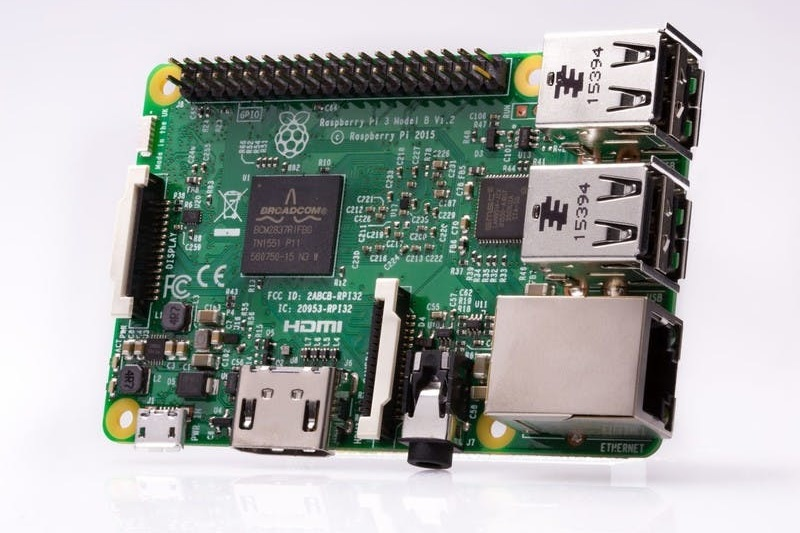
\includegraphics[scale=0.55]{pictures/raspberryPi3b.jpg}
	\caption{Raspberry Pi Modell 3b \textit{- Quelle: raspberrypi.org\cite{Foundation2020}}}
\end{figure}

\textbf{Servomotoren}\newline
	Servomotoren sind spezielle Elektromotoren, welche die Möglichkeit besitzen, die Winkelposition ihrer Motorwelle sowie die Drehgeschwindigkeit und Beschleunigung zu kontrollieren. Sie bestehen aus einem Elektromotor, der zusätzlich mit einem Sensor zur Positionsbestimmung ausgestattet ist.  Die durch den Sensor ermittelte Drehposition der Motorwelle wird kontinuierlich an eine, meist außerhalb des eigentlichen Motors angebrachte, Regelelektronik übermittelt, den so genannten Servoregler, welcher die Bewegung des Motors entsprechend einem oder mehreren einstellbaren Sollwerten, als auch Soll-Winkelposition der Welle oder Solldrehzahl in einem Regelkreis regelt.	
	\newline\newline	
\textbf{16-channel 12-bit Servo Driver}\newline
	Dieses Modul bietet eine Steuerung von mehreren Servo Motoren gleichzeitig. Durch eine externe Spannungquelle sind bis zu 16 5V Servo Motoren anschließbar.

\section{3D - Druck}
3D Druck ist eine Technologie die seit Jahren von der Industrie als auch von Privatandwendern betrieben, verbessert und erweitert wird. Diese Art des Druckens umfasst sämtliche Verfahren in denen Material Schicht auf Schicht aufeinander aufbauend gedruckt wird.
Für dieses Verfahren wird ein 3D Drucker benötigt. Ein handelsüblicher Filament (thermoplastische Kunststoffe in Drahtform) Drucker besitzt in der Standartvariante drei bis vier Achsenbewegungsmotoren, einen Extudermotor, ein Heizbett, ein Controllerboard, ein Hotend und einen Rahmen indem alle Bauteile verankert sind, sowie eine Spannungsquelle.
Für das Drucken von 3D Objekten sind neben einem Drucker auch Druckmaterial sowie ein Slicingprogramm nötig. Je nach Druckerart können verschiedenste Filamente verwendet werden. Das am meistverwendete Material ist PLA(Polylactide). Diese Polymere zählen zu den Polyestern und lassen sich am einfachsten drucken. \\
In dem Slicingprogramm werden die Modelle auf einem virtuellem Druckbett positioniert und in einzelne Schichten zerlegt. Je nach dem wie hoch eine Schicht ist, desto detaillierter ist das gedruckte Produkt. Aktuelle Drucker sind in der Lage eine Schichthöhe von 0,1 mm zu erreichen. Das bedeutet, dass für ein 1 mm hohes Objekt 10 Schichten für eine Schichthöhe von 0,1 mm verwendet werden müssen und für eine Schichthöhe von 0,2 nur 5. \\
Der Druckkopf(Hotend), aus dem das heiße Fillament kommt, bewegt sich im dreidimensionalen Raum(drei Achsen, X,Y,Z). Diese Bewegungen werden durch die Achsbewegungsmotoren ausgeführt. Um das Material in das Hotend(über 200 Grad heißer Metallblock mit Düsenspitze) zu drücken wird ein Extudermotor benötigt.
In dieser Beschreibung wurden Fused Deposition Modeling / Fused Filament Fabrication (FDM / FFF) besprochen. Daneben gibt es noch andere Druckerarten, wie zum Beispiel Stereolithographie (STL / SLA), bei welchem Flüssigharz und UV-Strahlen verwendet werden um Modelle zu drucken.
\subsection{Beispieldruck PLA}
Nachdem der Drucker die Datei mit dem gesliceten Druckmodel geladen hat, findet die Vorbereitung des Druckers automatisch statt.
Das Druckbett bzw. Heizbett wird auf $60^\circ\text{C}$ vorgeheizt, damit das Material besser an der Druckfläche haftet.
Währenddessen wird das Hotend auf eine Betriebstemperatur von ca  $215^\circ\text{C}$ erhitzt, damit das Material formbar wird und Schicht für Schicht aufgetragen werden kann.
Sind die Endtemperaturen erreicht, werden die einzelnen Befehle aus der geslicten Datei geladen. Diese beinhaltet Befehle für die Motoren.
Die gedruckte Schicht im Druckbett verhärtet sofort, sodass die nächst höhere Schicht auf eine stabile Oberfläche gesetzt werden kann.
\section{Android}
Android ist ein von Google Inc. entwickeltes und das meist verbreiteste Betriebsystem auf dem deutschen Markt\footnote{Stand März 2020 laufen ca. 80\% der verfügbaren Geräte mit einem Android Betriebssytem -\textit{Quelle: Statista.com, \glqq{}Vergleich der Marktanteile von Android und iOS am Absatz von Smartphones in Deutschland von Januar 2012 bis März 2020\grqq{}, 03.06.2020}\cite{Tenzer2020}}. Mittlerweile findet es nicht mehr nur in Smartphones, sondern auch in Smartwatches, Tablets und in Fernsehern Verwendung. Die App wurde auf der Version 8.1 (Oreo) entwickelt, ist aber trotzdem zu aktuelleren Versionen kompatibel. \\
Die aktuellste Android Version ist Android 10. Android 11 folgt im dritten Quartal 2020.
\chapter{Konzeption}
Bei dem Entwurf des Graphical User Interfaces (GUI) wurde sich an gängigen Fernsteuerungen aus der Spielbranche und dem Modellbau orientiert. Auf der linken sowie auf der rechten, unteren Seite des Displays, lässt sich die Position des Arms im dreidimensionalen Raum (3D) steuern. Im oberen Bereich der Anwendung befinden sich Konfigurationspunkte sowie der \glqq{}Switch\grqq{}\footnote{Ein Switch ist in Android ein Kippschalter mit 2 Zuständen}, welcher das Steuern des Greifers übernimmt. Die App sollte nur im \glqq{}Landscape\grqq{}-Modus, ausführbar sein, dies hat technische- und ergonomische Hintergründe. Dabei wurde Wert auf das Einhalten von aktuellen Konventionen, wie einem Settings Menü zum Festlegen von Serverport und -IP Adresse, als auch auf CISCO Standart Symbolen wie dem Netzwerk-Symbol geachtet. Des Weiteren wurde mit dem Erstellen von eigenen Scaleable Vector Graphics (SVG) die Intiutivität unterstützt und eine missverständliche Nutzung der Applikation ausgeschlossen.\\ \\

%Hier nun Konzeptidee vom Arm und Servercode

Für die Kommunikation zwischen der App und dem \glqq{}Roboterarm\grqq{} soll ein Server als Verbindungskomponennte verwendet werden. Mit diesem Konzept wird eine asynchrone Kommunikation zwischen Server und Client ermöglicht. Der Client, welcher als Sender von Daten dient, kann dem Server, welcher die Daten empfängt, direkt Daten übermitteln. Diese Verbindung wird durch einen TCP Socket gewährleistet. Die gesendeten Informationen der Applikation werden über die auf dem Raspberry PI vorhanden GPIO Pins an die Servomotoren mittels eines  \glqq{}16-channel 12-bit Servo Driver\grqq{} übertragen. Dieser Treiber ist Notwendig um eine konstante und ausreichende Spannungsquelle für die Motoren zu gewährleisten. Eine direkte Ansteuerung von mehr als einem Motor über die Spannungsquelle des Raspberry PI's ist ungenügend und lässt die Servomotoren zucken oder gar nicht reagieren.


\chapter{Implementierung}	
\section{Client}
Für die Entwicklung einer nativen Android App wird die Entwicklungsumgebung Android Studio benötigt. Des Weiteren wird für die Softwareversionsverwaltung auf die Plattform Github zurückgegriffen, wo der Quellcode des Projektes dokumentiert ist\footnote{https://github.com/JoProt/User-Interface-Project}. Aus dem Grund, dass die Verbindung zu dem Roboter Arm über das Internet realisiert wurde, ist es notwendig in dem Manifest der Anwendung die Internetberechtigung zu erteilen. \\
\begin{lstlisting}
<uses-permission android:name="android.permission.INTERNET" />
\end{lstlisting}

Damit ist es möglich auf das mobile Netz des Smartphones zuzugreifen. Um eine Verbindung aufzubauen, benötigt der Client, in diesem Fall die App, die Adresse und den Port des Hosts, in diesem Fall der Server auf dem Raspberry Pi. \\
Die Parameter für die Verbindung (IP und Port des Hosts), lassen sich dynmaisch (zur Laufzeit) in der App einsehen und anpassen. Dadurch ist es in der Theorie möglich mehrere Roboter nacheinander zu steuern. 
Damit das ankommende Signal welches die Knöpfen und der Switch senden, korrekt interpretiert wird, sendet die App einen eindeutigen, einstelligen Integer Code. Dadurch lassen sich die Bewegungen der Motoren durch den korrekten Knopf in der App abbilden. \\ \\
Da Pfeile als Bewegungsindikatoren im 3D Raum leicht missverstanden werden können, wurden eigene SVGs erstellt, welche die Bewegung des Arms verdeutlichen. 
\begin{figure}[h]
	\centering
	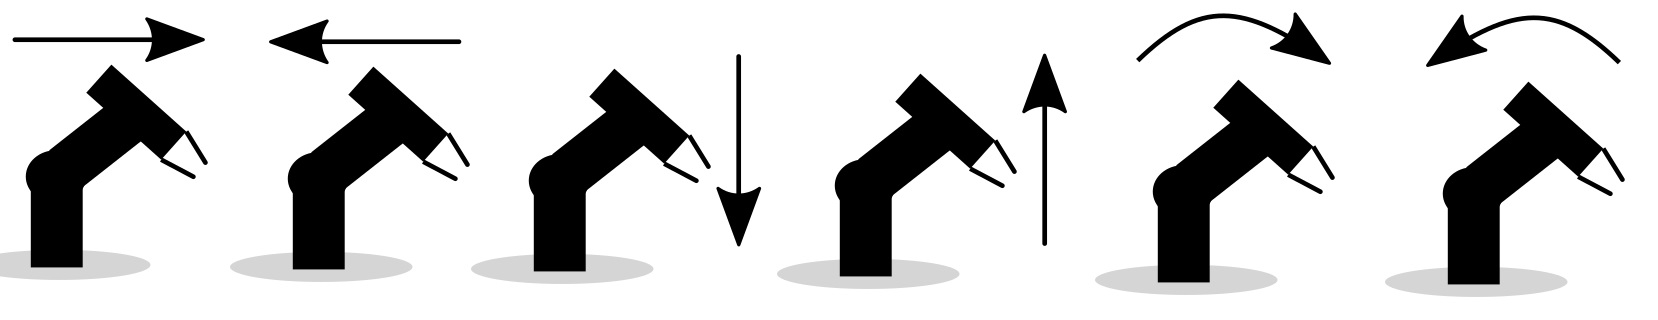
\includegraphics[scale=0.3]{pictures/robissvg.jpg}
	\caption{SVG der Knöpfe aus der App \textit{- Quelle: Eigene Darstellung}}
\end{figure}
\newpage
SVG hat den Vorteile, dass die Kanten und Formen in der Bildebene mathematisch berechnet werden. So lässt siche diese Grafik beliebig skalieren. \\
In Abbildung 4.1 sind die einzelnen Grafiken für die jeweilige Bewegung des Roboters aufgelistet, wobei $\leftarrow$ und $\rightarrow$ für Steuerung auf einer horizontal Linie, $\uparrow$ und $\downarrow$ für vertikale Bewegungen und $\curvearrowleft$ und $\curvearrowright$ für Bewegung um die eigene Hochachse verantwortlich sind.

\section{Roboterarm}
Der Arm wurde von einem selbstgebauten 3D-Drucker über 25 Stunden gedruckt und hat durch die Ungenauigkeit des Druckers und falschen Einstellungen einen leichten Verzug in den Bauteilen. Das bedeutet, die Greifzange hat ein leichtes Problem beim Schließen, dies würde sich mit neuen gedruckten Greifzangen-Bauteilen beheben lassen. Aus technischen Gründen ist dies nicht mehr möglich gewesen, da der Drucker derzeit einem technischen Defekt unterliegt.
Der Arm hat an vier Punkten die Servomotoren implementiert und kann sich dadurch wie in Abschnitt 4.1 beschrieben in mehrere Richtungen bewegen. Die Motorsteuerung funktioniert über ein 16-channel 12-bit Servo Driver-Board. Genaueres zu diesem Bauteil ist unter dem Abschnitt 2.1 zu lesen.
\newpage
\section{Server}
Für den Server und die Ansteuerung des Roboterarms wurde die Programmiersprache Python verwendet\cite{PiHandbuch}. Die Verbindung zum Server wird über eine Socket Verbindung gewährleistet, dass bedeutet, es wird eine direkte Verbindung zwischen Client und Server aufgebaut, die solange aktiv ist bis einer der beiden Partner die Verbindung trennt. Eine aktive Trennung findet in dieser Implementierung nur durch den Client statt. Wie im folgenden Codeauszug zu sehen ist wird eine Verbindung aufgebaut und gehalten. Es werden Daten empfangen, welche an die Roboterarmsteuerungsmethode weitergeleitet werden.
\begin{lstlisting}
# Server Init and Loop ---
serv = socket.socket(socket.AF_INET, socket.SOCK_STREAM)
serv.bind(('192.168.178.29', 5556))
serv.listen(5)
print("Server started")

while True:
    conn, addr = serv.accept()
    print ('client connected')
    from_client = ''
    while True:
        data = conn.recv(4096)
        if not data: break
        print (data.decode())
        handleData(data.decode())
    conn.close()
    print ('client disconnected')
\end{lstlisting}


In der Armsteuerung wird überprüft, welche Daten gesendet wurden. Intern wurde sich zuerst über eine passende Kommunikation ausgetauscht und danach wurden die jeweiligen Bewegungen per Zahl definiert. Beispielsweise wird Basis, welche das drehen nach links und rechts ermöglicht durch Integerwerte 7(links) und 8(rechts) definiert. Im folgenden Codeausschnitt wurde vorher überprüft ob es sich wirklich um eine Zahl handelt, dann wurde sie geparst und per \glqq{}if\grqq{}-Abfrage wird nun geprüft um welche Zahl es sich handelt. 
\newpage
\begin{lstlisting}
 if(number==8):
       if(servoPosBase+servoSteps<=maxServo):           
           servoPosBase+=servoSteps;
           kit.servo[2].angle = servoPosBase;
        
    if(number==7):
       if(servoPosBase-servoSteps>=minServo):           
           servoPosBase-=servoSteps;
           kit.servo[2].angle = servoPosBase;
\end{lstlisting}
Hierbei ist zu erkennen, dass der Mindest- und der Maximalwinkel des Servomoters als auch die Schrittgröße für ein Eingangssignal vorher definiert wurden. Dies dient dazu Fehler für die Motoren zu verhindern.  Mithilfe des ``ServoKit''-Packages ist es möglich eine vorgefertigte Ansteuerungsmethode zu verwenden \cite{Foundation2020}.


Wenn ein Datenstrom vom Client gesendet wird, wird dieser durch den Server validiert und weitergereicht um einen Motor des Armes zu bewegen.


\chapter{Fehlschläge}
%(\textbf{hier musst du unbedingt noch Quellen angeben. Du sagst selbst im Text das du vorher kein Wissen hattest, aber worher hast du das denn jetzt genimmen? such bitte noch min. eine weitere Quelle raus. am Besten 2.  Wenn du willst, kannst du mein Raspberry Pi Buch auch als Quelle nutzen dann gebe ich dir die daten durch.}) \\ \\ \\ \\
Für die Server-Arm Steuerung wurden mehrere Ansätze ausgetestet. Zum Einen war das Wissen, wie solche Motoren und Systeme funktionieren nicht vorhanden. Dadurch sind Probleme wie zuckende, nicht reagierende Servomotoren und Fehlansteuerungen entstanden. Erst bei der Betrachtung, dass die Spannungsquelle ungenügend sein könnte, wurde recherchiert\cite{I2C} und Lösungen betrachtet. 

 
\chapter{Zusammenfassung}	
In diesem Projekt haben wir uns mit den Grundlagen der Entwicklung eines User Interfaces auseinandergesetzt und eine ansprechende und intuitiv zu bedienende App entwickelt. Mit Hilfe unseres Wissens aus weiteren Modulen, wie zum Beispiel \glqq{}Programmierung Mobiler Endgeräte\grqq{} und \glqq{}Echtzeit- und Netzwerktprogrammierung\grqq{}, war es uns möglich, eine Android Anwendung zu schreiben um den Roboter Arm zusteuern. 
\\
In der Zeit der Digitalisierung, in der Computer immer mehr Teil unseres Alltags werden ist es das Ziel, dass die Maschinen für den Menschen eine Arbeitserleichterung und keine zusätzliche Last werden. Deshalb ist es umso wichtiger, mit einem qualitativem User Interface zu arbeiten. Dieses vergleichsweise kleine Projekt hat uns gezeigt, wie aufwendig der Prozess der Gestaltung einer hochwertigen Oberfläche ist.\\ \\
Gerade dann, wenn eine Anwendung veröffentlicht und von mehreren Menschen genutzt wird, ist es wichtig, dass es das Leben erleichtert und nicht verkompliziert.
\pagenumbering{roman}

	%-----------------------------------------------------------------------------
	% Literaturverzeichnis einf�gen, 
	% Nutzung der BibTeX-Technologie --> literatur.bib 
	%-----------------------------------------------------------------------------

	
	\bibliographystyle{unsrtdin}		%  Stil des Literaturverzeichnisses (hier nach DIN 1505)
	\bibliography{literatur}			% gibt Datei mit der Literatur an
	
	\nocite{*}						% damit alle in der DB enthaltende Eintr�ge bearbeitet werden
	

	%-----------------------------------------------------------------------------
	% Verzeichnisse
	%-----------------------------------------------------------------------------
	\listoffigures						% Bildverzeichnis einf�gen

	%-----------------------------------------------------------------------------
	% Anhang
	%-----------------------------------------------------------------------------	
	\appendix
	% Auch hier sind Gliederungen aller \chapter, \section
	

	%-----------------------------------------------------------------------------
	% Selbstst�ndigkeitserkl�rung
	%-----------------------------------------------------------------------------	
	\chapter*{Selbstst\"andigkeitserkl\"arung}
	\addcontentsline{toc}{chapter}{Selbstst\"andigkeitserkl\"arung}
	\rhead{Selbstst\"andigkeitserkl\"arung} % rechts oben in der Kopfzeile Chapter darstellen
	Hiermit erkl\"aren wir, dass wir die hier vorliegende Arbeit selbstst\"andig,
	ohne unerlaubte fremde Hilfe und nur unter Verwendung der aufgef\"uhrten
	Hilfsmittel angefertigt haben.

	\begin{tabular}{p{10cm}p{13cm}}
		\\
  		\\
  		\\
  		\\
  		Wismar, den \today \\
  		---------------------------------------  & ------------------------------ \\
  		Ort, Datum & Unterschrift
	\end{tabular}
	

\end{document}							% Ende des Dokuments
%-----------------------------------------------------------------------------
